% Copyright 2020-2022 Robert Bosch GmbH

% Licensed under the Apache License, Version 2.0 (the "License");
% you may not use this file except in compliance with the License.
% You may obtain a copy of the License at

% http://www.apache.org/licenses/LICENSE-2.0

% Unless required by applicable law or agreed to in writing, software
% distributed under the License is distributed on an "AS IS" BASIS,
% WITHOUT WARRANTIES OR CONDITIONS OF ANY KIND, either express or implied.
% See the License for the specific language governing permissions and
% limitations under the License.

\hypertarget{description-robotframework-testcase-settings}{%
\section{\rfwcore\ Testcase Settings:}
\label{description-robotframework-testcase-settings}}

For the whole test execution:

\begin{itemize}

\item Project/Variant (can be overwritten by argument \rlog{--variant} or
  \rlog{--config} of
  \href{https://github.com/test-fullautomation/robotframework-testresultwebapptool}{RobotResults2DB}
  tool when importing):

\begin{robotcode}
Metadata    project     ${Project_name}
\end{robotcode}

\item Versions (can be overwritten by argument \rlog{--versions} or
  \rlog{--config} of
  \href{https://github.com/test-fullautomation/robotframework-testresultwebapptool}{RobotResults2DB}
  tool when importing):

\begin{robotcode}
Metadata    version_hw     ${Software_version}
Metadata    version_hw     ${Hardware_version}
Metadata    version_test   ${Test_version}
\end{robotcode}
\end{itemize}

For the Suite/File information:
\begin{itemize}

\item Description/Documentation:

\begin{robotcode}
Documentation   ${Suite_description}
\end{robotcode}

\item Author:

\begin{robotcode}
Metadata   author   ${Author_name}
\end{robotcode}

\item Component (can be overwritten by argument \rlog{--config} of
  \href{https://github.com/test-fullautomation/robotframework-testresultwebapptool}{RobotResults2DB} 
  tool when importing):
  
\begin{robotcode}
Metadata   component   ${Component_name}
\end{robotcode}

\item Test Tool - framework and python version, e.g \textbf{Robot Framework
  3.2rc2 (Python 3.9.0 on win32)}:

\begin{robotcode}
Metadata   testtool   ${Test_tool}
\end{robotcode}

\item Test Machine:

\begin{robotcode}
Metadata   machine   %{COMPUTERNAME}
\end{robotcode}

\item Tester:

\begin{robotcode}
Metadata   tester   %{USER}
\end{robotcode}

\end{itemize}

For test case information:

\begin{itemize}

\item Issue ID:

\begin{robotcode}
[Tags]   ISSUE-${ISSUE_ID}
\end{robotcode}

\item Testcase ID:

\begin{robotcode}
[Tags]   TCID-${TC_ID}
\end{robotcode}

\item Requirement ID:

\begin{robotcode}
[Tags]   FID-${REQ_ID}
\end{robotcode}
\end{itemize}


\hypertarget{description-sample-robotframework-testcase}{%
\section{Sample \rfwcore\ Testcase:}
\label{description-sample-robotframework-testcase}}

For test case management, we need some tracable information such as
version, testcase ID, component, ... to manage and track testcase(s) on
RQM.

So, this information can be provided in \rcode{Metadata} (for the whole
testsuite/execution info: version, build, ...) and \rcode{{[}Tags{]}}
information (for specific testcase info: component, testcase ID,
requirement ID, ...).

Sample \rfwcore\ testcase with the neccessary information for importing to
RQM:

\begin{robotcode}[caption=Sample \rfwcore\ testcase,
                  linebackgroundcolor=\hlcode{12,13,14}]
*** Settings ***
# Test execution level
Metadata   project        ROBFW              # Project/Variant
Metadata   version_sw     SW_VERSION_0.1     # Software version
Metadata   version_hw     HW_VERSION_0.1     # Hardware version
Metadata   version_test   TEST_VERSION_0.1   # Test version

# File/Suite level
Documentation             This is description for robot test file
Metadata    author        Tran Duy Ngoan (RBVH/ECM1)
Metadata    component     Import_Tools
Metadata    testtool      Robot Framework 3.2rc2 (Python 3.9.0 on win32)
Metadata    machine       %{COMPUTERNAME}
Metadata    tester        %{USER}

*** Test Cases ***
Testcase 01
   [Tags]   ISSUE-001   TCID-1001   FID-112   FID-111
   Log       This is Testcase 01

Testcase 02
   [Tags]   ISSUE-RTC-003   TCID-1002   FID-113
   Log       This is Testcase 01
\end{robotcode}

\begin{boxhint} {Hint}
You don't need to define above highlighted \rcode{Metadata}(\rcode{testtool},
\rcode{machine} and \rcode{tester}) with \rfw\ because 
\href{https://github.com/test-fullautomation/robotframework-testsuitesmanagement}{RobotFramework\_Testsuites}
library will handle these definitions within \rcode{Suite Setup}.
\end{boxhint}

\newpage
\hypertarget{description-display-on-webapp}{%
\section{Display on WebApp:}\label{description-display-on-webapp}}

When the \emph{output.xml} file(s) is importing sucessfully to database,
the result for that execution will be available on
\href{https://github.com/test-fullautomation/testresultwebapp}{TestResultWebApp}.

Above settings in robot testcase will be reflect on \textbf{Dashboard}
(General view) and \textbf{Data table} (Detailed view) as below figures:

Execution result metadata:

\begin{figure}[h!]
  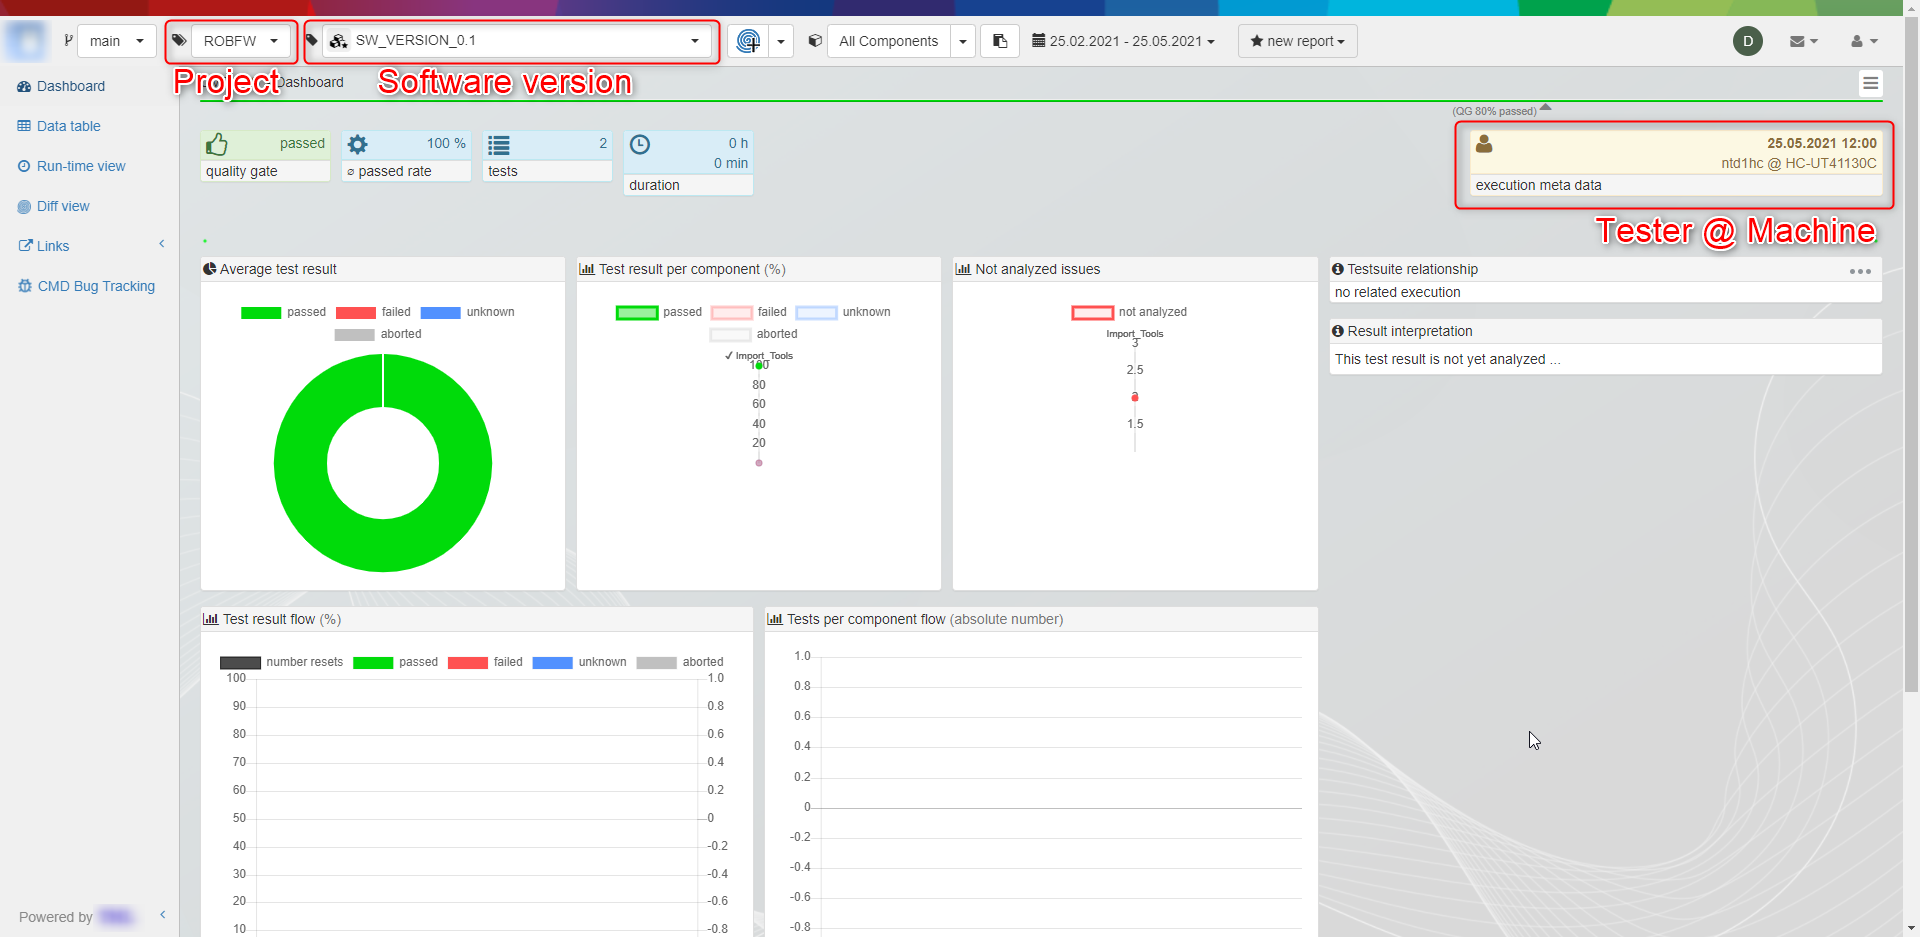
\includegraphics[width=1\linewidth]{./pictures/Dashboard.png}
  \caption{Dashboard view}
\end{figure}

Suite/File metadata and Testcase information:

\begin{figure}[h!]
  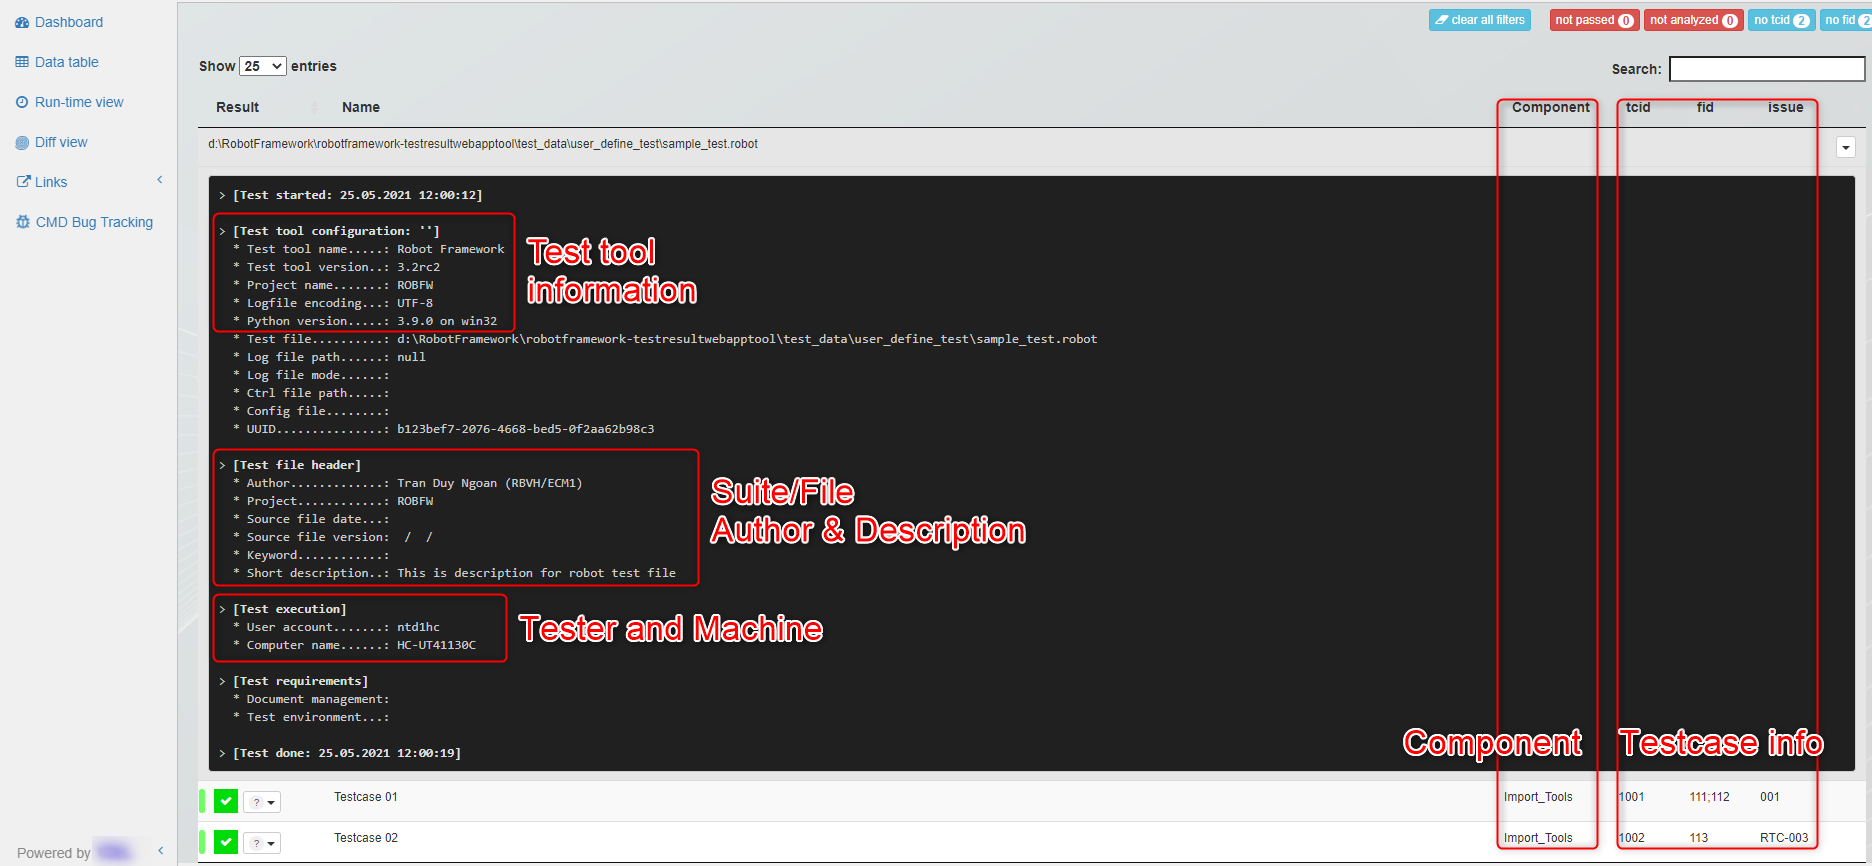
\includegraphics[width=1\linewidth]{./pictures/Datatable.png}
  \caption{Datatable view}
\end{figure}


\hypertarget{description-notes}{%
\section{Notes:}\label{description-notes}}

When above settings is missing, that leads to the missing information in
the \emph{output.xml}.

Some required fields for management will be set to default value when
importing with
\href{https://github.com/test-fullautomation/robotframework-testresultwebapptool}{RobotResults2DB}
tool:

\begin{itemize}
\tightlist
\item \rlog{Project}: will be set to default value \pcode{ROBFW} if not defined.

\item \rlog{Software version}: will be set to execution time
  \pcode{\%Y\%m\%d\_\%H\%M\%S} as default value.

\item \rlog{Component}: will be set to default value \pcode{unknown} if not
  defined.
\end{itemize}

But, you can provide them as command arguments when executing the
\href{https://github.com/test-fullautomation/robotframework-testresultwebapptool}{RobotResults2DB}
tool with below optional arguments (refer its
\href{https://github.com/test-fullautomation/robotframework-testresultwebapptool\#usage}{usage}):

\begin{itemize}
\item \rlog{--variant VARIANT}

  To specify the {Project/Variant} information.

\item \rlog{--versions VERSIONS}

  To specify the {Software version} information.

\item \rlog{--config CONFIG}

  Provide a configuration json file \pcode{CONFIG} which helps:

  \begin{itemize}
  \item To configure the {Project/Variant}, {Software version} information
    (lower priority than above commandline arguments)

  \item To create a mapping between testcase folder and {Component}
    information which is display on
    \href{https://github.com/test-fullautomation/testresultwebapp}{TestResultWebApp}.
  \end{itemize}

  Sample configuration json file:

\begin{pythoncode}
{
   "component"  : {
                  "cli"       : "robot/cli",
                  "core"      : "robot/core",
                  "external"  : "robot/external",
                  "keywords"  : "robot/keywords",
                  "libdoc"    : "robot/libdoc",
                  "output"    : "robot/output",
                  "parsing"   : "robot/parsing",
                  "reboot"    : "robot/reboot",
                  "rpa"       : "robot/rpa",
                  "running"   : "robot/running",
                  "std_lib"   : "robot/standard_libraries",
                  "tags"      : "robot/tags",
                  "test_lib"  : "robot/test_libraries",
                  "testdoc"   : "robot/testdoc",
                  "tidy"      : "robot/tidy",
                  "variables" : "robot/variables"
   },
   "version_sw" : "Atest",
   "variant"    : "ROBFW"
}
\end{pythoncode}
\end{itemize}
